\section{Semiconductors}\label{sec:Semiconductors}
\subsection{Depletion Layer}\label{subsec:Depletion_Layer}
\begin{definition}[Depletion Layer]\label{def:Depletion_Layer}
  The \emph{depletion layer} is the location in the \PNJunction{} where the two differently-doped sides meet.
  Here, there is a barrier of the opposing carrier on each side.
  This is visualized in \Cref{fig:Depletion_Layer}.
\end{definition}

\begin{figure}[h!tbp]
  \centering
  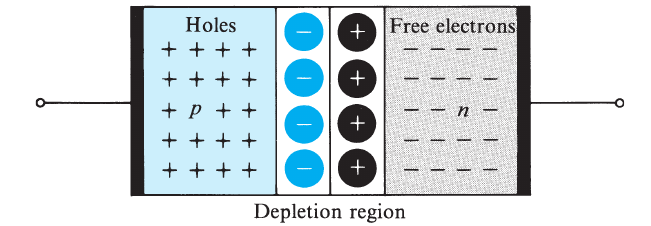
\includegraphics[scale=0.5]{./Depletion_Layer.png}
  \caption{Depletion Layer (\cite[p.~150]{sedraTextbook7})}
  \label{fig:Depletion_Layer}
\end{figure}


%%% Local Variables:
%%% mode: latex
%%% TeX-master: "../ECE_311-Engineering_Electronics-Reference_Sheet"
%%% End:
